\textbf{Example 1}

For the railway network shown above, the grader would make the following function call:

\texttt{ find\_shortcut(4, [10, 20, 20], [0, 40, 0, 30], 10)}

The optimal solution is to build the express line between stations $1$ and $3$, as shown below.

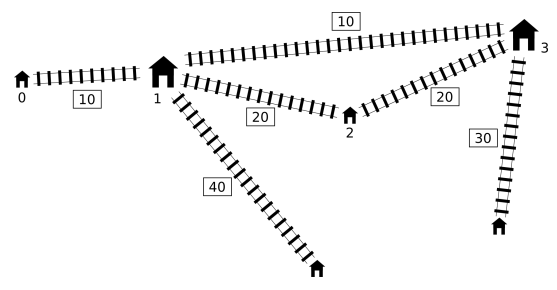
\includegraphics[scale=0.9]{2.png}

The diameter of the new railway network is $80$ centimeters, so the function should return $80$.

\textbf{Example 2}

The grader makes the following function call:

\texttt{find\_shortcut(9, [10, 10, 10, 10, 10, 10, 10, 10], [20, 0, 30, 0, 0, 40, 0, 40, 0], 30)}

The optimal solution is to connect stations $2$ and $7$, in which case the diameter is $110$.

\textbf{Example 3}

The grader makes the following function call:

\texttt{find\_shortcut(4, [2, 2, 2], [1, 10, 10, 1], 1)}

The optimal solution is to connect stations $1$ and $2$, reducing the diameter to $21$.

\textbf{Example 4}

The grader makes the following function call:

\texttt{ find\_shortcut(3, [1, 1], [1, 1, 1], 3) }

Connecting any two stations with the express line of length $3$ does not improve the initial diameter of the railway network which is $4$.
